\documentclass[tikz,border=5pt]{standalone}
\usepackage{tikz}
\usepackage{amsmath}
\usetikzlibrary{arrows.meta}
\definecolor{nebula}{HTML}{6366F1}
\definecolor{spark}{HTML}{14B8A6}
\definecolor{ink}{HTML}{334155}
\begin{document}
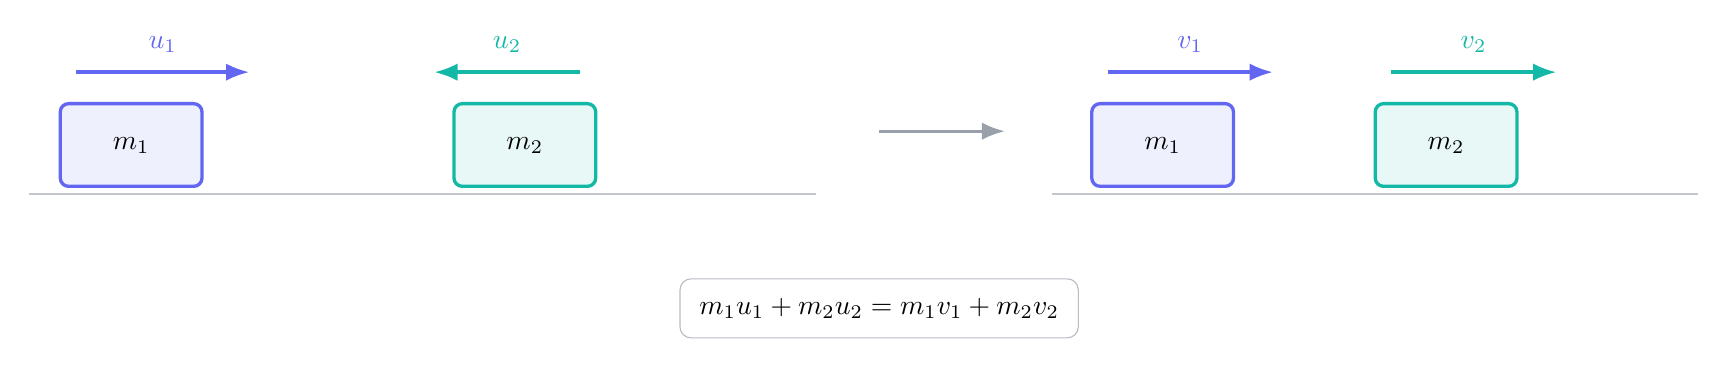
\begin{tikzpicture}[font=\sffamily,>=Latex]
  \draw[ink!30,thick] (-5,-.8)--(5,-.8);
  \draw[rounded corners=3pt,very thick,nebula,fill=nebula!10] (-4.6,-.7) rectangle (-2.8,.35);
  \node at (-3.7,-.18) {$m_1$};
  \draw[->,very thick,nebula] (-4.4,.75)--(-2.2,.75) node[midway,above=3pt] {$u_1$};
  \draw[rounded corners=3pt,very thick,spark,fill=spark!10] (.4,-.7) rectangle (2.2,.35);
  \node at (1.3,-.18) {$m_2$};
  \draw[->,very thick,spark] (2.0,.75)--(.15,.75) node[midway,above=3pt] {$u_2$};
  \draw[->,ink!50,very thick] (5.8,0)--(7.4,0);
  \draw[ink!30,thick] (8,-.8)--(16.2,-.8);
  \draw[rounded corners=3pt,very thick,nebula,fill=nebula!10] (8.5,-.7) rectangle (10.3,.35);
  \node at (9.4,-.18) {$m_1$};
  \draw[->,very thick,nebula] (8.7,.75)--(10.8,.75) node[midway,above=3pt] {$v_1$};
  \draw[rounded corners=3pt,very thick,spark,fill=spark!10] (12.1,-.7) rectangle (13.9,.35);
  \node at (13,-.18) {$m_2$};
  \draw[->,very thick,spark] (12.3,.75)--(14.4,.75) node[midway,above=3pt] {$v_2$};
  \node[draw=ink!35,rounded corners=4pt,fill=white,inner sep=7pt] at (5.8,-2.25)
    {$m_1u_1+m_2u_2=m_1v_1+m_2v_2$};
\end{tikzpicture}
\end{document}
